\documentclass[12pt]{article}
\usepackage[utf8]{inputenc}
\usepackage[T2A]{fontenc}
\usepackage[russian]{babel}
\usepackage{amsmath}
\usepackage{amssymb}
\usepackage{dsfont}
\usepackage[dvipsnames]{xcolor}
\usepackage{setspace}
\usepackage{multirow}
\usepackage[a4paper, outer=1.5cm, inner=1.5cm, top=1cm, bottom=1cm]{geometry}
\usepackage{graphicx}
\usepackage{skull}
\usepackage{wasysym}
\usepackage{float}
\graphicspath{{.images/}}
\usepackage{hyperref}
\hypersetup{colorlinks=true, linkcolor=blue, filecolor=magenta, urlcolor=cyan}
\usepackage[firstpage]{draftwatermark}
\SetWatermarkText{
    $\qquad\qquad\qquad\qquad\qquad$\parbox{7cm}{\begin{center}
    
\includegraphics[width = 0.08\textwidth]{lion-logo.png}\bigskip\\~\bigskip\\~\vspace{-24mm}\\~\end{center}}
}
\SetWatermarkAngle{0}
\SetWatermarkScale{1.5}
\usepackage{etoolbox}

\newtoggle{ifsolved}
\newtoggle{needhelp}
\newcounter{num}
\setcounter{num}{1}

\newcommand{\newnum}{\par\textbf{\textnumero\arabic{num}}\stepcounter{num}}
\newcommand{\sol}{\vspace{3mm}\par\textbf{Решение: }}
\newcommand{\ans}{\vspace{3mm}\par\textbf{Ответ: }}
\newcommand{\hint}{\vspace{3mm}\par\textbf{Подсказка: }}
\newcommand{\mode}[1]{
\ifstrequal{#1}{0}{\togglefalse{ifsolved}\togglefalse{needhelp}}{\ifstrequal{#1}{1}{\togglefalse{ifsolved}\toggletrue{needhelp}}{\ifstrequal{#1}{2}{\toggletrue{ifsolved}\togglefalse{needhelp}}{\toggletrue{ifsolved}\toggletrue{needhelp}}}}} %if 0 - if 1 - if 2 - else
%\newenvironment{problem}[8]{%#1, #2, #3
%\parbox{\linewidth}{\vspace{4mm}\ifstrequal{#4}{(лёгкая)}{\newnum\textbf{.}}{\newnum\textbf{*.} } \\ #5}
%\iftoggle{ifsolved}{\sol #6}{}
%\iftoggle{ifsolved}{\ans #7}{}
%\iftoggle{needhelp}{\hint #8}{}}

\newenvironment{problem}[8]{%#1, #2, #3
\parbox{\linewidth}{\vspace{5mm}\ifstrequal{#4}{(лёгкая)}{\newnum\textbf{.}}{\newnum\textbf{*.} } \\ #5}
\iftoggle{ifsolved}{\sol #6}{}

\iftoggle{ifsolved}{\parbox{\linewidth}{\ans #7}}{}
\iftoggle{needhelp}{\parbox{\linewidth}{\hint #8}}{}}

\newenvironment{mylist} %custom list
{ \begin{itemize}
    \setlength{\itemsep}{0pt}
    \setlength{\parskip}{0pt}
    \setlength{\parsep}{0pt}     }
{ \end{itemize}                  }

\newenvironment{homeass}[1]{\vspace*{-1.5cm}
\iftoggle{ifsolved}{
    \section*{\center{Решение домашнего задания к #1.}}
}{
    \section*{\center{\textcolor{Sepia}{Домашнее задание к #1}}}
} \vspace{7mm}\large}

\parindent=0pt
\pagestyle{empty}
%$\!$[\arabic{class}.\arabic{num}]
%\ifnumcomp{\value{counter}}{>}{1}{true}{false}
%\definecolor{Gray}{gray}{0.9}
%\definecolor{mypink}{RGB}{219, 48, 122}
%\newcolumntype{g}{>{\columncolor{Gray}}p{2.8cm}}

\begin{document}
\large
\mode{7}
%0 for problems without hints
%1 for problems + hints
%2 for problems + solutions + answers
%else: show all

{\centering\section*{СПИСОК ЗАДАЧ}}

{\centering\subsection*{\smallskip\\\textcolor{green}{\textbf{Полезные вещи, которые можно и нужно копипастить:}}}}

\subsection*{\textcolor{Emerald}{\textbf{Полезные шпаргалки по LaTeXу:}}}

\textbf{Пример вставки рисунка:}

\begin{minipage}{\linewidth}
    \begin{minipage}{0.54\linewidth}
    см. рисунок справа\\
    Текст к собственно пикче, примерно всегда это либо развёрнутое описание, либо большая часть решения задачи --- стремимся экономить пространство, если это можно сделать.
    \end{minipage}
    \hspace{0.05\linewidth}
    \begin{minipage}{0.4\linewidth}
    \begin{figure}[H] 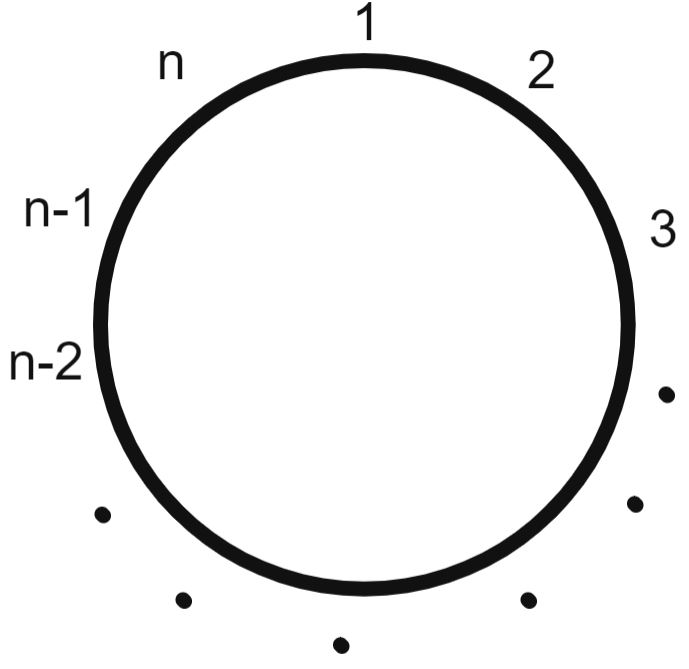
\includegraphics[width=\linewidth]{sol3} %тут поменять имя пикчи
    \end{figure}
    \end{minipage}
\end{minipage}

\textbf{Дефолтные математические знаки и символы:}\\
$\geqslant$,
$\leqslant$,
$a^{b}$,
$x_{i}$,
$\sqrt{a}$,
$\frac{a}{b}$,
$\displaystyle \frac{a}{b}$,
$\cdot$
$\;\Rightarrow\;$,
$\;\Leftrightarrow\;$,
$1{,}2$.
О промежутках:
$a\!b$,
$a\,b$,
$a\:b$,
$a\;b$,
$a\quad b$.

\textbf{Стандартные система и совокупность уравнений / неравенств:}\\
$\left\{
\begin{aligned}
f(x) &= 0 \\
g(x) &= 1
\end{aligned}\right.$

$\left[\begin{aligned}
&\left\{\begin{aligned}
f(x) &\geqslant a \\
g(x) &= b
\end{aligned}\right.\\
&\left\{\begin{aligned}
f(x) &< a \\
g(x) &= -b
\end{aligned}\right.
\end{aligned}\right.$

\subsection*{\textcolor{Emerald}{\textbf{Не математическое, но полезное:}}}
% комментарий в любом месте документа, который нигде не будет видно. Можно использовать для написания заметок-вопросов по задачам
\textbf{Пример таблицы:}

\begin{tabular}{|c|c|c|}
\hline
    $a$ & $b$ & текст
\\\hline
    $c$ & $d$ & мораль
\\\hline
\end{tabular}\\

\textbf{Отступы:} между\smallskip\\ строками\medskip\\ \textbf{Тире} --- это три дефиса.\\
\textbf{Списки:}
\begin{mylist}
\item [$\bullet$] это был пункт а
\item [2)] а это уже пункт номер 2 с изменённым заголовком
\end{mylist}

\subsection*{\textcolor{Emerald}{\textbf{Всё, неупомянутое выше (или если просто что-то не так):}}}
\begin{mylist}
\item [$\bullet$] Решение отдельных вопросов касательно ТеХа нужно искать в \href{https://www.mccme.ru/free-books/llang/newllang.pdf}{Львовском}.

\item [$\bullet$] Найти произвольный символ, который нужен, можно в \href{http://detexify.kirelabs.org/classify.html}{Detexify}.

\item [$\bullet$] Если возникли сомнения при решении, ответ практически ко всем задачам можно проверить с помощью \href{https://www.wolframalpha.com/}{WolframAlpha}.

\item [$\bullet$] Если в задаче нужно создать картинку, то лучше пока отложить эту задачу. Все графики планируется централизованно нарисовать (или перерисовать) в геогебре.

\item [\textcolor{brown}{\textbf{!!}}] Важно ставить \textcolor{red}{\textbf{$\spadesuit$}}
(или просто red) в тело задачи в случае серьёзных вопросов к решению и какой-то вопиющей лажи.

\item [\textcolor{brown}{\textbf{!!}}] Важно ставить \textcolor{olive}{\textbf{$\spadesuit$}}
(или просто olive) в тело задачи в случае не самого удачного текста и кривых отступов.
\end{mylist}

\subsection*{\textcolor{Violet}{\textbf{Комментарии:}}}% а также невидимые комментарии - так можно оставлять заметки-вопросы прямо в задаче, чтобы потом было понятно, в чём вопрос.
\begin{mylist}
\item [$\skull$] Переставлять задачи местами --- очень плохая идея.

\item [$\smiley$] При двойном клике по тексту pdf справа происходит автоматический переход к этому месту в латех-коде, а для обратного перехода можно нажать стрелку вправо (висит сверху между pdf и латех-кодом).

\item [$\smiley$] Если есть размышления, дописывать red/olive к задаче или не дописывать, то лучше всё-таки дописать.

\item [$\skull$] Самое плохое, что можно сделать --- написать в любое поле из трёх (НаписанноеРешение/ВерныйОтвет/Подсказка) только половину того, что надо, никак это не отметить, и потом пойти дальше.\\ Нужно в этот момент писать red/olive в случайном месте задачи, чтобы потом вычислить это с помощью Ctrl+F по всему документу (и это то, что потом будет делаться долго и тщательно)
\end{mylist}

\newpage
\setcounter{num}{74}

\hypertarget{6.3}{{\centering\section*{\bigskip\\\textcolor{Blue}{\hyperlink{start2}{\textcolor{Blue}{6.3}} Умножение и деление дробей.}\vspace{-5mm}}}}

\begin{problem}{Умножение дробей и нахождение доли от числа.}{6.3.1}{6K}{(лёгкая)}
{В июле килограмм яблок стоил $80$ рублей. В августе яблоки подешевели на пятую часть цены, а в сентябре подешевели ещё на четверть цены. Сколько рублей стоил килограмм яблок в сентябре?}
{\textcolor{olive}{\textbf{$\spadesuit$}}После того, как яблоки в августе подешевели на пятую часть,  цена от прежней станет $\frac45$   стоимости, то есть $ 80\cdot\frac45=64$. В сентябре  подешевела еще на четверть, следовательно, цена от последней  станет $\frac34$ стоимости, то есть $ 64\cdot\frac34=48$. Таким образом, килограмм яблок в сентябре стоил $48$ рублей.}
{Килограмм яблок в сентябре стоил $48$ рублей.}{Для начала необходимо выяснить, сколько рублей составила стоимость яблок в августе.}
\end{problem}

\begin{problem}{Умножение дробей и нахождение доли от числа.}{6.3.1}{6S}{(лёгкая)}
{К Васе пришло в гости 4 друга, и они вместе сели есть клубничный пирог.\\ Первый друг получил $\frac{1}{5}$ пирога, второй~--- $\frac{1}{4}$ остатка, третий~--- $\frac{1}{3}$ нового остатка.\\ Оставшуюся часть пирога Вася разделил поровну с четвёртым другом.\\ Кому досталась большая часть?}
{После того, как первый друг получит $\frac15$ пирога, ещё $\frac45$ пирога останется. Второй друг получит четверть от этого, то есть $\frac45 \cdot \frac14 = \frac15$ пирога. После этого останется $\frac45 - \frac15 = \frac35$ пирога. Треть нового остатка для третьего друга --- это $\frac35 \cdot \frac13 = \frac15$, остаётся $\frac25$ пирога, которые Вася и четвёртый друг делят поровну (каждый получит $\frac15$ пирога). То есть в итоге каждый друг (и Вася) получил по $\frac15$ пирога: пирог разделили поровну, большая часть никому не досталась.}
{Пирог был разделён поровну между всеми пятью друзьями.}{Какая часть пирога останется после того, как первый друг получит свой кусок? А после того, как кусок возьмёт второй друг?}
\end{problem}

\begin{problem}{Умножение дробей и нахождение доли от числа.}{6.3.1}{6S}{(лёгкая)}
{Автомобиль прошёл за 4 ч 180 км. В первый час он прошёл $\frac{4}{15}$ всего пути, во второй~--- $\frac{5}{8}$ того, что прошёл в первый час, в третий~--- вдвое меньше пройденного за первые два часа вместе, а в четвёртый~--- весь остальной путь.\\ Сколько километров прошёл автомобиль за четвёртый час?}
{Так как в первый час он прошёл $\frac{4}{15}$ от всего расстояния, то есть от 180 км, это составляет $180\cdot\frac{4}{15} = \frac{180\cdot4}{15} = \frac{36\cdot4}{3} = 48$ километров. За второй час он прошёл $\frac58$ от этого, то есть $48\cdot\frac58 = 30$ км. Таким образом, всего к этому моменту он проехал $48 + 30 = 78$ км. За третий час он прошёл вдвое меньше, то есть $78 : 2 = 39$ километров. Значит, за первые 3 часа он проехал $78 + 39 = 117$ километров. Поскольку в последний час он проехал всё оставшееся расстояние, это означает, что за четвёртый час он проехал $180 - 117 = 63$ км.}
{За последний, четвёртый час, автомобиль прошёл 63 километра.}{Для начала необходимо выяснить, сколько километров проехал этот автомобиль за первый час своего движения.}
\end{problem}

\begin{problem}{Умножение дробей и нахождение доли от числа.}{6.3.1}{6S}{*}
{a) Половина от трети числа~--- 100. Что это за число?
\\b) Сколько будет полторы трети от 100?}
{\textcolor{olive}{\textbf{$\spadesuit$}}\smallskip\\а) Пусть неизвестное число $X$. Тогда треть от числа будет $\frac{X}{3}$. Половина от трети означает $\frac{1}{2}\cdot\frac{X}{3}=\frac{X}{3\cdot2}=\frac{X}{6}$. Сказано, что половина от трети это 100. Составим уравнение: \smallskip\\
$\frac{X}{6}=100$\smallskip\\
$\frac{X}{6}=100\cdot6$\smallskip\\
$X=600$\smallskip\\
b) Представим треть от $100$ дробью: $\frac{100}{3}$, а полтора как $\frac{3}{2}$. Тогда полтора от трети 100 будет  $\frac{3}{2}\cdot\frac{100}{3}=\frac{100\cdot3}{2\cdot3}=\frac{100}{2}=50$.
}
{а) 600 b) 50}{а) Выразить треть от числа и умножить на половину. b) Выразить треть от числа и умножить на полтора.}
\end{problem}

\begin{problem}{Взаимно обратные числа.}{6.3.3}{6S}{*}
{Вода, превращаясь в лёд, увеличивается в объёме на $\frac{1}{9}$ часть.\\
На какую часть уменьшится объём льда при таянии?}
{После превращения воды в лёд объём льда будет составлять $\frac{10}{9}$ от начального объёма воды. Понятно, что после того, как лёд растает обратно, его объём будет равным начальному объёму. На какую часть он уменьшится?\\ Исчезнет $\frac19$ из $\frac{10}{9}$, то есть часть в десять раз меньшая, чем объём льда.\\ Получается, что кусок льда при таянии в объёме уменьшится на $\frac{1}{10}$.}
{Кусок льда при таянии уменьшится на $\frac{1}{10}$ своего объёма.}{Какую часть составляет величина уменьшения от объёма льда?}
\end{problem}

\begin{problem}{Деление дробей и нахождение числа по его доли.}{6.3.4}{6K \textcolor{red}{\textbf{$\spadesuit$}}}{(лёгкая)}
{\vspace{-10mm}\\\begin{minipage}{\linewidth}
    \begin{minipage}{0.57\linewidth}
    \vspace{10mm}
    Фигуры А, B, C и D на рисунке справа являются квадратами. Периметр квадрата А равен 12 см и составляет $\frac{3}{5}$ от периметра квадрата В.\\ Чему (в см$^{2}$) равна площадь квадрата D?

    \end{minipage}
    \hspace{0.03\linewidth}
    \begin{minipage}{0.38\linewidth}
        \begin{figure}[H]
        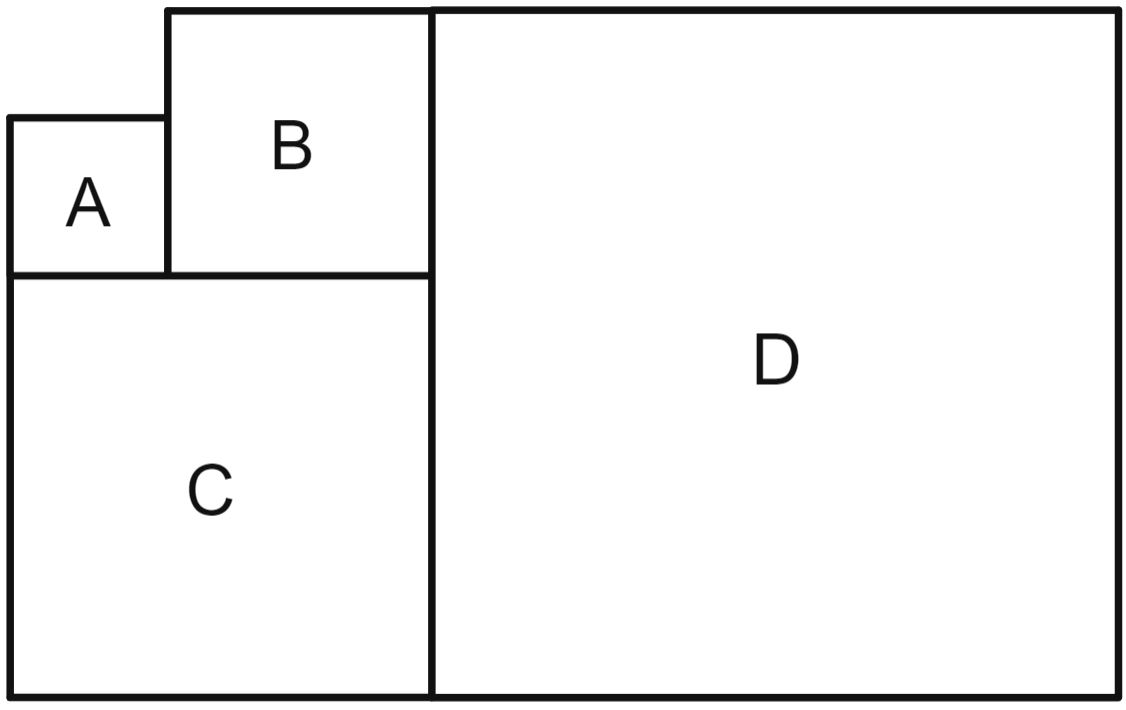
\includegraphics[width=\linewidth]{6K-1}
        \end{figure}
    \end{minipage}
\end{minipage}}
{Несложно подметить, что раз периметр квадрата А известен и равен 12 см, то каждая его сторона равна 3 см. 12 см составляет $\frac35$ от другого числа, являющегося величиной периметра квадрата B. Это означает, что периметр квадрата B равен $12 : \frac35 = 12\cdot \frac53 = 60 : 3 = 20$ см. Но тогда сторона квадрата B равна $20 : 4 = 5$ см. Значит, сторона квадрата C равна $3 + 5 = 8$ см (поскольку она складывается из сторон квадратов A и B). Cторона квадрата D, в свою очередь, складывается из сторон квадратов B и C и равна $5 + 8 = 13$ см. Площадь квадрата равна произведению стороны квадрата на себя: $S_D = 13\cdot 13 = 169$ см$^2$.}
{Площадь квадрата D равна 169 см$^2$.}{Чему равны сторона квадрата A и периметр квадрата B?}
\end{problem}

\begin{problem}{Деление дробей и нахождение числа по его доли.}{6.3.4}{6S}{(лёгкая)}
{Кирпич весит 2кг и ещё треть собственного веса. Сколько весит кирпич?}
{\vspace{-5mm}\\\begin{minipage}{\linewidth}
    \begin{minipage}{0.59\linewidth}
    ~\vspace{4mm}\\
    Если кирпич весит 2 килограмма и ещё треть кирпича, то это означает, что 2 килограмма --- это оставшиеся $\frac23$ кирпича.\smallskip
    \end{minipage}
    \hspace{0.05\linewidth}
    \begin{minipage}{0.35\linewidth}\begin{figure}[H] 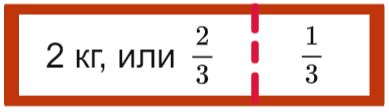
\includegraphics[width=\linewidth]{sol74}\end{figure}\end{minipage}
\end{minipage}
Следовательно, треть кирпича весит вдвое меньше этого, а именно 1 килограмм. Значит, весь кирпич весит $2 + 1 = 3$ килограмма.}
{Кирпич весит три килограмма.}{Какую часть кирпича составляют упомянутые 2 килограмма?}
\end{problem}

\begin{problem}{Деление дробей и нахождение числа по его доли.}{6.3.4}{6S}{(лёгкая)}
{Краб весит 2кг и ещё $\frac{6}{7}$ своего веса. Сколько весит краб?}
{ \textcolor{olive}{\textbf{$\spadesuit$}}Если краб весит 2 килограмма и ещё $\frac67$ от веса, то это означает, что 2 килограмма --- это оставшиеся $\frac17$ краба. Следовательно, $\frac17$ краба  весит в 7 раз меньше полного веса. Значит, весь краб весит $2 \cdot\ 7 = 14$ кг.}
{Краб весит 14 килограмм.}{Какую часть краба составляют упомянутые 2 килограмма?}
\end{problem}

\begin{problem}{Деление дробей и нахождение числа по его доли.}{6.3.4}{6S}{(лёгкая)}
{Мама перед уходом положила на стол сливы и сказала трём сыновьям, чтобы они, вернувшись из школы, поделили их поровну. Первым пришёл Миша, он взял треть слив, и ушёл. Потом вернулся из школы Петя, взял треть от лежавших на столе слив и тоже ушёл. Затем пришёл Коля и тоже взял треть слив от числа слив, которые он увидел. Сколько слив оставила мама, если Коля взял 4 сливы?}
{Нам известно только то, сколько слив взял Коля. Раз он взял 4 сливы, то по его мнению, это треть от всех слив --- значит, в тот момент, когда он пришёл, на столе было $4\cdot3 = 12$ слив. Сколько в таком случае слив досталось Пете?\\
12 слив лежало на столе уже после того, как он забрал свою треть, а значит, эти 12 слив --- это две трети от того, что лежало на столе до его появления. То есть Петя забрал $12 : 2 = 6$ слив, а до его прихода на столе лежало $12 + 6 = 18$ слив. Аналогично, Миша забрал слив вдвое меньше, чем оставил: то есть Миша взял $18 : 2 = 9$ слив, а до его возвращения из школы слив было $18 + 9 = 27$ штук.\\
Следовательно, мама оставила 27 слив.}
{Мама оставила 27 слив.}{Сколько слив лежало на столе до прихода Коли?\\ Какую часть составляет это число от количества слив, которые лежали на столе до возвращения Пети из школы?}
\end{problem}

\begin{problem}{Деление дробей и нахождение числа по его доли.}{6.3.4}{6S}{(лёгкая)}
{Среди математиков каждый седьмой~--- философ, а среди философов каждый девятый~--- математик. Кого больше, философов или математиков?}
{НаписанноеРешение}
{ВерныйОтвет}{А сколько тех, кто одновременно и философ, и математик?}
\end{problem}

\begin{problem}{Деление дробей и нахождение числа по его доли.}{6.3.4}{6S}{(не лёгкая)}
{Когда база отпустила магазинам $\frac{5}{12}$ имевшегося у неё запаса крупы, на базе осталось на 5 центнеров больше половины всего запаса крупы.\\ Сколько крупы было на базе?}
{После того, как база отпустила магазинам $\frac{5}{12}$ запаса крупы, у неё осталось $1 - \frac{5}{12} = \frac{7}{12}$ запаса крупы. На сколько это больше половины? $\frac{7}{12} - \frac12 = \frac{7}{12} - \frac{6}{12} = \frac{1}{12}$. Это означает, что на базе осталась половина всего запаса крупы, и ещё $\frac{1}{12}$ имевшегося запаса крупы. Следовательно, $\frac{1}{12}$ всего запаса крупы --- 5 центнеров, а значит всего на базе было $5\cdot 12 = 60$ центнеров крупы (6 тонн).}
{На базе было 6 тонн крупы.}{На сколько текущее количество крупы на базе больше половины общего запаса крупы?}
\end{problem}

\begin{problem}{Деление дробей и нахождение числа по его доли.}{6.3.4}{6S}{(лёгкая)}
{Когда турист проехал $\frac{3}{8}$ всего пути между двумя городами, то до половины пути ему осталось проехать 15 км. Найти расстояние между городами.}
{В тот момент, когда турист проехал $\frac38$ пути между городами, до половины пути ему осталось проехать $\frac12 - \frac38 = \frac48 - \frac38 = \frac18$ пути. Значит $\frac18$ пути --- 15 км, а весь путь в 8 раз длиннее и расстояние между городами равно $15 \cdot 8 = 120$ км.}
{Расстояние между городами равно $120$ км.}{Какую часть пути туристу осталось проехать до половины?}
\end{problem}

\begin{problem}{Деление дробей и нахождение числа по его доли.}{6.3.4}{6S}{(лёгкая)}
{Если из $\frac{3}{4}$ неизвестного числа вычесть 10 и полученную разность умножить на 5, то получится 100. Найти это число.}
{После умножения на 5 получилось 100. Значит, до умножения на 5 было число в 5 раз меньшее. Делим на 5. $100 : 5 = 20$. Это число получилось после того, как было вычтено 10. Значит, до вычитания было число на 10 больше. Прибавляем 10. $20 + 10 = 30$. Получились $\frac34$ неизвестного числа.\\ Если $\frac34$ некоторого числа равны 30, то само число равно $30 : \frac34 = 30 \cdot \frac{4}{3} = \frac{30\cdot4}{3} = 40$.}
{Это число равно 40.}{Что за число было до умножения на 5? А до вычитания 10?}
\end{problem}

\begin{problem}{Деление дробей и нахождение числа по его доли.}{6.3.4}{6S}{*}
{Если к неизвестному числу прибавить $\frac{3}{4}$ его да ещё 40, то получится 180.\\ Найти это число.}
{\textcolor{olive}{\textbf{$\spadesuit$}}После того, как прибавили 40, получилось 180. Значит, до сложения число было на 40 меньше 180. То есть $ 180 - 40 = 140$. Исходя из условия, это сумма неизвестного числа и его  $\frac34$. Отсюда мы делаем вывод, что 140 это 1$\frac34$ неизвестного числа. Другими словами, 140 это  $\frac74$  числа. Следовательно, искомое значение это 140 : $\frac74 = 140 \cdot \frac47 = 20\cdot 4 = 80$.}
{Это число 80.}{Проанализировать шаги действий с числом и двигаться в обратном направлении.}
\end{problem}

\begin{problem}{Деление дробей и нахождение числа по его доли.}{6.3.4}{6S}{(лёгкая)}
{Сумма трёх чисел равна $64\frac{4}{5}$; первое число в $2\frac{1}{2}$ раза, а второе в $3\frac{1}{4}$ раза больше третьего. Найти эти числа.}
{\textcolor{olive}{\textbf{$\spadesuit$}}Пусть первое число будет $X$, второе число будет $Y$, третье $Z$. Так как сказано, что первое число в $2\frac{1}{2}$ раза больше третьего, то $X=2\frac{1}{2}Z$. Второе в $3\frac{1}{4}$ раза больше третьего, следовательно $Y=3\frac{1}{4}Z$. Сумма трёх чисел равна $64\frac{4}{5}$, следовательно, $X+Y+Z=64\frac{4}{5}$. Исходя из этого: \smallskip\\
$3\frac{1}{4}Z+2\frac{1}{2}Z+Z=64\frac{4}{5}$\smallskip\\
$6\frac{3}{4}Z=64\frac{4}{5}$\smallskip\\
$\frac{27}{4}Z=\frac{324}{5}$\smallskip\\
$Z=\frac{324}{5}\cdot\frac{4}{27}=\frac{12\cdot4}{5}=\frac{48}{5}=9\frac{3}{5}$\smallskip\\
Так как $X=2\frac{1}{2}Z$ , то $X=2\frac{1}{2}\cdot9\frac{3}{5}=\frac{5}{2}\cdot\frac{48}{5}=\frac{48}{2}=24$\smallskip\\
Так как $Y=3\frac{1}{4}Z$, то $Y=3\frac{1}{4}\cdot9\frac{3}{5}=\frac{13}{4}\cdot\frac{48}{5}=\frac{13\cdot12}{5}=\frac{156}{5}=31\frac{1}{5}$

} 
{Первое число $24$, второе $31\frac{1}{5}$, а третье $9\frac{3}{5}$.}{Составить уравнение и выразить через третье число остальные неизвестные.}
\end{problem}

\begin{problem}{Деление дробей и нахождение числа по его доли.}{6.3.4}{6S}{*}
{Сумма трёх чисел равна $56\frac{3}{8}$. Первое число больше второго в $1\frac{1}{2}$ раза, а второе составляет $\frac{1}{2}$ третьего числа. Найти эти числа.}
{НаписанноеРешение}
{ВерныйОтвет}{Подсказка}
\end{problem}

\begin{problem}{Деление дробей и нахождение числа по его доли.}{6.3.4}{6S}{*}
{Сумма четырёх чисел равна $33\frac{3}{4}$. Второе число составляет $\frac{1}{2}$ первого; третье составляет $\frac{1}{2}$ второго; четвёртое составляет $\frac{1}{2}$ третьего. Найти эти четыре числа.

}
{НаписанноеРешение}
{ВерныйОтвет}{Подсказка}
\end{problem}

\begin{problem}{Деление дробей и нахождение числа по его доли.}{6.3.4}{6S}{(лёгкая)}
{В книге четыре рассказа. Первый рассказ занимает 12 страниц, что составляет $\frac{2}{3}$ второго рассказа. Третий рассказ занимает $\frac{5}{6}$ суммы страниц первых двух рассказов вместе. Какую часть книги занимает четвёртый расссказ, если всего в книге 64 страницы?}
{Раз первый рассказ составляет $12$ страниц, и эти 12 страниц равны $\frac23$ второго рассказа, то во втором рассказе $12 : \frac23 = \frac{\textcolor{gray}{12}\cdot3}{\textcolor{gray}{2}} = 18$ страниц. Поскольку про количество страниц в третьем рассказе известно, что оно составляет часть от суммы страниц первых двух страниц, то отметим, что первые два рассказа вместе занимают $12 + 18 = 30$ страниц. $\frac56$ от этого количества~--- это $30 \cdot \frac56 = \frac{\textcolor{gray}{30}\cdot5}{\textcolor{gray}{6}} = 25$.\\
Таким образом, третий рассказ занимает 25 страниц, а значит вместе первые три рассказа занимают $30 + 25 = 55$ страниц. Оставшиеся $64 - 55 = 9$ страниц будут заняты четвертым рассказом, поскольку других рассказов в этой книге нет.\\
Это означает, что четвёртый рассказ составляет $\frac{9}{64}$ книги.}
{Четвёртый рассказ составляет $\frac{9}{64}$ книги.}{Найди число страниц во всех рассказах (по очереди).}
\end{problem}

\begin{problem}{Деление дробей и нахождение числа по его доли.}{6.3.4}{6S}{(лёгкая)}
{Автомобиль в первый час прошёл $\frac{2}{7}$ расстояния между городами, во второй~--- $\frac{7}{13}$ оставшегося расстояния и в третий~--- остальные 90 км.\\ Найти расстояние между городами.}
{НаписанноеРешение}
{ВерныйОтвет}{Подсказка}
\end{problem}

\begin{problem}{Деление дробей и нахождение числа по его доли.}{6.3.4}{6S}{(лёгкая)}
{Когда турист прошёл $\frac{3}{10}$ всего пути, то до середины пути ему осталось пройти ещё $4\frac{1}{2}$ км. Найти длину всего пути.}
{НаписанноеРешение}
{ВерныйОтвет}{Подсказка}
\end{problem}

\begin{problem}{Деление дробей и нахождение числа по его доли.}{6.3.4}{6K}{(лёгкая)}
{Расставь знаки арифметических действий так, чтобы уравнение стало верным: $$\;\:\displaystyle \frac12 \phantom{-\,} \frac13 \phantom{-\,} \frac14 \phantom{-\,} \frac16 = 1\frac23.$$

}
{Можно отметить, что $1\frac23 = \frac53$. Вариантов ответа тут целых три: $$\displaystyle \frac12 \cdot \frac13 + \frac14 : \frac16 = 1\frac23 \qquad \frac12 - \frac13 + \frac14 : \frac16 = 1\frac23\qquad \frac12 + \frac13 : \frac14 - \frac16 = 1\frac23.$$}
{Подходящие способы расставить знаки (их три штуки) указаны выше.}{$1\frac23 = \frac53$; $\;\frac53 = \frac43 + \frac13 = \frac32 + \frac16$.}
\end{problem}

\begin{problem}{Деление дробей и нахождение числа по его доли.}{6.3.4}{6K}{(лёгкая)}
{Расставь знаки арифметических действий так, чтобы уравнение стало верным: $$\;\:\displaystyle \frac12 \phantom{-\,} \frac13 \phantom{-\,} \frac14 \phantom{-\,} \frac16 = 0.$$

}
{После аккуратного перебора (на самом деле, всего возможно $4\cdot4\cdot4 = 64$ варианта расставить знаки), можно найти следующие два решения:
$$\displaystyle \frac12 : \frac13 - \frac14 : \frac16 = 0, \qquad \frac12 - \frac13 \cdot \frac14 : \frac16 = 0.$$}
{Есть два решения: $\quad\displaystyle \frac12 : \frac13 - \frac14 : \frac16 = 0, \qquad \frac12 - \frac13 \cdot \frac14 : \frac16 = 0.$}{Есть два варианта ответа.}
\end{problem}

\begin{problem}{Деление дробей и нахождение числа по его доли.}{6.3.4}{6K}{(лёгкая)}
{Расставь знаки арифметических действий так, чтобы уравнение стало верным: $$\;\:\displaystyle \frac12 \phantom{-\,} \frac13 \phantom{-\,} \frac14 \phantom{-\,} \frac16 = 1\frac{11}{24}.$$

}
{Поскольку в ответе в итоге дробь со знаменателем 24, можно догадаться, что между $\frac14$ и $\frac16$ стоит умножение. Дальше ответ легко подбирается:
$$\displaystyle \frac12 : \frac13 - \frac14 \cdot \frac16 = 0.$$}
{Решение выглядит следующим образом: $\quad\displaystyle \frac12 : \frac13 - \frac14 \cdot \frac16 = 0.$}{Если известно, что в ответе~--- дробь со знаменателем 24, то какой знак стоит между $\frac14$ и $\frac16$?}
\end{problem}

\begin{problem}{Деление дробей и нахождение числа по его доли.}{6.3.4}{6K}{*}
{Расставь знаки арифм. действий так, чтобы уравнение стало верным: $$\;\:\displaystyle \frac12 \phantom{-\,} \frac13 \phantom{-\,} \frac14 \phantom{-\,} \frac16 = 2\frac14.$$

}
{НаписанноеРешение}
{% :*:
}{Подсказка}
\end{problem}

\begin{problem}{Деление дробей и нахождение числа по его доли.}{6.3.4}{6S}{(лёгкая)}
{Если к $\frac{2}{7}$ неизвестного числа прибавить 162, то получится $\frac{5}{7}$ того же числа.\\ Найди это число.}
{Так как сначала мы имели $\frac27$ некоторого числа, а после прибавления получили $\frac57$ этого числа, это означает, что было прибавлено ровно $\frac37$ этого числа.\\ То есть, $\frac{3}{7}$ этого числа равны 162.\\ В таком случае $\frac17$ этого числа втрое меньше и равна $162 : 3 = 54$.\\ Исходное неизвестное число в 7 раз больше и равно $54 \cdot 7 = 350+28 = 378$.}
{Это число~--- 378.}{Какую часть числа составляет прибавленная величина?}
\end{problem}

\begin{problem}{Деление дробей и нахождение числа по его доли.}{6.3.4}{6K}{*}
{Родители вместе с детьми пошли собирать ягоды, а когда вернулись и стали считать, кто сколько собрал, выяснили, что все ягоды, которые собрал Петя (четверть от общего количества всех собранных ягод)~--- незрелые.\\ Когда родители сказали об этом маленькому Пете, он очень обиделся и выкинул в окошко половину своего ведёрка с ягодами. Какую часть теперь составляют незрелые ягоды среди всех собранных (а не рассыпанных) ягод?}
{НаписанноеРешение}
{ВерныйОтвет}{Подсказка}
\end{problem}

\end{document}